\documentclass[12pt]{elsart}
\usepackage{amsmath}
\usepackage{amssymb}
\usepackage{program}
\usepackage{graphicx}
\newcommand{\field}[1]{\mathbb{#1}}
\usepackage[letterpaper,top=0.75in, bottom=0.75in, left=1in, right=1in]{geometry}
\usepackage[table]{xcolor}
\usepackage{wrapfig}


\usepackage{algorithm}
\usepackage{algpseudocode}

%%%%%%%%%%%%%%%%%%%%%%%%%%%%%%%%%%%%%%%%%Space to make more readable!
%\vspace{10 mm}
%%%%%%%%%%%%%%%%%%%%%%%%%%%%%%%%%%%%%%%%%Take out later!

\begin{document}

\pagestyle{empty}

\begin{center}
\Large  CS3343 Analysis of Algorithms Fall 2017 \\
\large {\bf Homework 6}\\
\normalsize Due 11/3/17 before 11:59pm (Central Time)
\end{center}

{\bf 1.  Franchise Restaurants (5 points)}

A fast food company is considering a bunch of bids to open franchises on a road and they want to develop an algorithm to decide which to accept.

For each of the $n$ miles along the road, the bid for that location is recorded (if there is no bid it is recorded as $0$).  The company wants to accept the bids which maximizes their total earnings.  One extra caveat is that two franchises must be at least $3$ miles apart (for example if you accept the bid at mile $5$ then you can't accept the bids at miles $3,4,6,7$).

\hspace*{0.5cm}  \begin{tabular}{ |l|l|l|l|l|l|l|l|l|l| }
  \hline
   Mile: & 1 & 2 & 3 & 4 & 5 & 6 & 7 & 8 & 9 \\
  \hline
  Bid: &   50,000 & 60,000 & 30,000 & 45,000 & 40,000 & 10,000 & 40,000 & 0 & 45,000 \\
  \hline
\end{tabular}

   \begin{enumerate}
      \item (1 point) Example:  For the bids given above, which would you accept to maximize the earnings? (in this case, $n=9$)\\
          I would accept the bids at miles 2, 5, and 9 for the maximum total of 145,000.
      \item (2 points) Let $E(n)$ denote your maximum earnings for the bids in the first $n$ miles.  Give a recursive definition of $E$:
   \begin{enumerate}
      \item Base case \\(Hint: this will occur when $n=0$ since there are no bids to consider).\\
          $E(0) = 0$
      \item Recursive case \\(Hint: compare the total value obtained from accepting the $n\textsuperscript{th}$ bid to the total value obtained from not accepting the $n\textsuperscript{th}$ bid).
          \begin{flalign*}
            E(n) &= \max\begin{cases}
              E(n-1) &\\
              \max\limits_{1 \leq i \leq n-3} (E(i) + b[n]) &
            \end{cases}&
          \end{flalign*}
   \end{enumerate}
      \item (2 points) Give pseudo-code for an algorithm which uses memoization to compute $E(n)$ based on the above recurrence (assume you are passed an array $b$ of the bids).\\
          \begin{algorithm}
            \caption{int getMaxProfits(int $n$, int[] $b$)}
            \begin{algorithmic}
                \State let $p[0..n]$ be a new array
                \For{$i = 0$ {\bf to} $n$}
                    \State $p[i] = -1$;
                \EndFor
                \State {\bf return} getMaxProfitsAux($n$, $b$, $p$);
            \end{algorithmic}
          \end{algorithm}
\newpage
          \begin{algorithm}
            \caption{int getMaxProfitsAux(int $n$, int[] $b$, int[] $p$)}
            \begin{algorithmic}
                \If{$p[n] \geq 0$}
                    \State {\bf return} $p[n]$;
                \EndIf
                \State $m = -1$;
                \For{$i = n - 3$; $i \geq 1$; $i--$}
                    \State $m =$ max(getMaxProfitsAux($n - 1$), getMaxProfitsAux($i) + b[n])$;
                \EndFor
                \State $p[n] = m$;
                \State {\bf return} $m$;
            \end{algorithmic}
          \end{algorithm}
   \end{enumerate}

{\bf 2.  Inventory Management (7 points)}

Suppose you are playing a video game.  In this game you can only carry a limited amount of items.  Every item has a value and your goal is to maximize the total value of items you are carrying.  

Specifically, you are choosing which of $m$ items to carry where item number $i$ has value $v[i]$ (for your recurrence/pseudo-code you can assume you are passed the item values  in an array, $v$, of size $m$).  

\begin{enumerate}
   \item Suppose you can only carry $n$ items of the $m$ available.
   \begin{enumerate}
      \item (1 point) Example: Let $n=3$, $m=5$.  If the item values are $v=\{5,30,17,32,40\}$ which $3$ should you choose to carry?\\
          I would choose to carry the items numbered 2, 4, and 5 for a maximum value of 102.
      \item (1 point) Give a short description of a greedy algorithm which maximizes your total value for any given $n$,$m$, and $v$.\\
          The algorithm would, at each step $i$ through the $m$ items, choose that item if $n$ items have not been chosen yet or replace the minimum of the chosen $n$ items so far with the $i$th item if $v[i]$ is greater than that minimum item of the $n$ chosen so far.
   \end{enumerate}

   \item Suppose, the game is updated so that every item, $i$, now has weight, $w[i]$, in kilograms (you can assume you are passed the item weights in an array, $w$, of size $m$).  You can only carry $n$ kilograms of weight.
   \begin{enumerate}
      \item (1 point) Example: Let $n=15$, $m=5$.  If the item values are $v=\{5,30,17,32,40\}$ and the item weights are $w=\{2,4,3,6,15\}$ which should you choose to carry?  Which would your greedy algorithm choose to carry?\\
          I would choose to carry the first 4 items for a maximum value of 84 and weight of 15. My greedy algorithm would select the items with the highest value obeying the constraints of weight, which would select the 5th item only for a value of 40 and weight of 15.
      \item (2 points) Let $V(n,m)$ denote your maximum total value for any given $n$, $m$, $v$, and $w$.  Give a recursive definition of $V$:
   \newpage
   \begin{enumerate}
      \item Base case \\(Hint: your base case will occur when $m=0$ since you have no items left to consider).\\
          $V(n,0) = 0$ and $V(0,m) = 0$
      \item Recursive case \\(Hint: compare the total value obtained from taking the $m\textsuperscript{th}$ item to the total value obtained from not taking the $m\textsuperscript{th}$ item).
          \begin{flalign*}
              V(n, m) &=\begin{cases}
                V(n, m - 1) & w[m] > n\\
                \max\begin{cases}
                  V(n, m - 1)\\
                  V(n - w[m], m - 1) + v[m]
                \end{cases} & otherwise
              \end{cases}&
          \end{flalign*}
   \end{enumerate}
      \item (2 points) Based on your recurrence, write the pseudo-code for a dynamic programming algorithm to compute the maximum total value (you can use bottom up dynamic programming or memoization).\\
      \begin{algorithm}
        \caption{int getMaxValue(int $n$, int $m$, int $v$[], int $w$[])}
        \begin{algorithmic}
          \State let $p[0..m][0..n]$ be a new array
          \For{$i = 0$ {\bf to} $m$}
              \For{$j = 0$ {\bf to} $n$}
                  \If{$i == 0$ {\bf or} $j == 0$}
                      \State $p[i][j] = 0$;
                  \ElsIf{$w[i - 1] > j$}
                      \State $p[i][j] = p[i - 1][j]$;
                  \Else
                      \State $p[i][j] = max(p[i - 1][j]$, $p[i - 1][j - w[i - 1]] + v[i - 1])$;
                  \EndIf
              \EndFor
          \EndFor
          \State {\bf return} $p[m][n]$;
        \end{algorithmic}
      \end{algorithm}
   \end{enumerate}
\end{enumerate}

\newpage

{\bf 3.  DFS and BFS (6 points)}

For the following problems, assume that vertices are ordered alphabetically in the adjacency lists (thus you will visit adjacent vertices in alphabetical order).

   \begin{enumerate}
      \item (2 points) Execute a Breadth-First Search on the graph $G_1$, starting on vertex $a$. Specifiy the visit times for each node of the graph.
          \begin{figure}[h]
            \centering 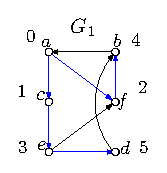
\includegraphics[width=.45\textwidth]{Graph-02}
          \end{figure}
      \item (2 points) Execute a Depth-First Search on the graph $G_1$, starting on vertex $a$. Specifiy the visit and finish times for each node of the graph
   \begin{enumerate}
      \item (1 point) For each edge in your graph identify whether it is a tree edge, back edge, forward edge, or a cross edge.
          \begin{figure}[h]
            \centering 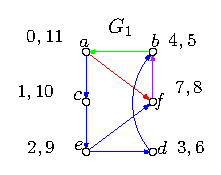
\includegraphics[width=.45\textwidth]{Graph-03}
          \end{figure}
      \item (1 point) Which edges would you remove to make your graph into a DAG?  (hint: use your edge classification to justify your choice)\\
          I would remove all back edges, because a cycle is defined when a path exists where the first and last vertices are the same. Thus, there would be an edge from a vertex to its ancestor in the path and, by definition, that is a back edge in the edge classifications of a depth first search. Thus if you remove all back edges, you remove all cycles.
   \end{enumerate}

   \end{enumerate}


{\bf 4.  Prim's Algorithm (4 points)}

(4 points) Run Prim’s algorithm on the graph $G_2$, with start vertex $a$. Assume that vertices are ordered alphabetically. 

For each step of the algorithm specify the current vertex weights (you can use a table to represent this data).  Draw the minimum spanning tree the algorithm finds. 

\begin{figure}[h]
	\centering 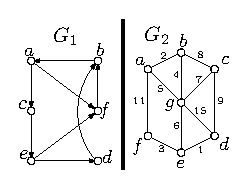
\includegraphics[width=.45\textwidth]{Graph-01}
\end{figure}

\begin{tabular}{|l|l|l|l|l|l|l|l|}
  \hline
  step & $a$ & $b$ & $c$ & $d$ & $e$ & $f$ &  $g$\\
  \hline
  1 & 0 & $\infty$ & $\infty$ & $\infty$ & $\infty$ & $\infty$ & $\infty$\\
  \hline
  2 & \cellcolor{blue!25} 0 & 2 & $\infty$ & $\infty$ & $\infty$ & 11 & 5\\
  \hline
  3 & \cellcolor{blue!25} 0 & \cellcolor{blue!25} 2 & 8 & $\infty$ & $\infty$ & 11 & 4\\
  \hline
  4 & \cellcolor{blue!25} 0 & \cellcolor{blue!25} 2 & 7 & 15 & 6 & 11 & \cellcolor{blue!25} 4\\
  \hline
  5 & \cellcolor{blue!25} 0 & \cellcolor{blue!25} 2 & 7 & 1 & \cellcolor{blue!25} 6 & 3 & \cellcolor{blue!25} 4\\
  \hline
  6 & \cellcolor{blue!25} 0 & \cellcolor{blue!25} 2 & 7 & \cellcolor{blue!25} 1 & \cellcolor{blue!25} 6 & 3 & \cellcolor{blue!25} 4\\
  \hline
  7 & \cellcolor{blue!25} 0 & \cellcolor{blue!25} 2 & 7 & \cellcolor{blue!25} 1 & \cellcolor{blue!25} 6 & \cellcolor{blue!25} 3 & \cellcolor{blue!25} 4\\
  \hline
  8 & \cellcolor{blue!25} 0 & \cellcolor{blue!25} 2 & \cellcolor{blue!25} 7 & \cellcolor{blue!25} 1 & \cellcolor{blue!25} 6 & \cellcolor{blue!25} 3 & \cellcolor{blue!25} 4\\
  \hline
\end{tabular}

\begin{wrapfigure}{r}{0.5\textwidth}
  \centering 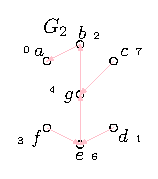
\includegraphics[width=.45\textwidth]{Graph-04}
\end{wrapfigure}

\end{document}